\documentclass[conference]{IEEEtran}
\IEEEoverridecommandlockouts
% The preceding line is only needed to identify funding in the first footnote. If that is unneeded, please comment it out.
\usepackage{cite}
\usepackage{amsmath,amssymb,amsfonts}
%\usepackage{algorithmic}
\usepackage{graphicx}
\usepackage{textcomp}
\usepackage{xcolor}

%\usepackage{algorithm}git add
\usepackage{algpseudocode}
\usepackage{arevmath}     % For math symbols
\usepackage{bbm}

\usepackage[linesnumbered,ruled,vlined]{algorithm2e}
\newcommand\mycommfont[1]{\footnotesize\ttfamily\textcolor{blue}{#1}}
\SetCommentSty{mycommfont}
\SetKwInput{KwInput}{Input}                % Set the Input
\SetKwInput{KwOutput}{Output}              % set the Output

% Math font
%\usepackage{mathpazo}
\usepackage{fourier}

\DeclareMathOperator*{\argmax}{arg\,max}

% Enable subfigures
\graphicspath{ {./pictures/} }
\usepackage{subcaption}
\captionsetup{compatibility=false}

\def\BibTeX{{\rm B\kern-.05em{\sc i\kern-.025em b}\kern-.08em
    T\kern-.1667em\lower.7ex\hbox{E}\kern-.125emX}}
\begin{document}

\title{Imbalanced Dataset Techniques to Improve Classification of Uneven Class Distributions\\
}

\author{\IEEEauthorblockN{Miguel Jiménez Aparicio}
\IEEEauthorblockA{
Atlanta, USA\\
maparicio6@gatech.edu}
\and
\IEEEauthorblockN{Belén Martín Urcelay}
\IEEEauthorblockA{
San Sebastián, Spain \\
burcelay3@gatech.edu}
\and
\IEEEauthorblockN{Cristian Gómez Peces}
\IEEEauthorblockA{
Atlanta, USA \\
cpeces3@gatech.edu}
}

\maketitle

\begin{abstract}
This document analyzes the impact of imbalanced datasets on machine learning classifiers and discusses several techniques to deal with them. The results are applied to train a Twitter fake account detection algorithm where the performance of these techniques is compared. The paper shows how state-of-the-art ensemble and cost-sensitive classifiers lead to a substantial increase in F1-score compared to traditional classifiers, while both true and empirical risks decrease.
\end{abstract}

\begin{IEEEkeywords}
imbalance, undersampling, oversampling, boosting, bagging, cost-sensitive.
\end{IEEEkeywords}

\section{Introduction}
	\subsection{Motivation}
	Many canonical machine learning algorithms used for classification assume that the number of objects in the respective classes is roughly the same. However, in reality, classes are rarely represented equally. Class distribution skews are not only common, but many times expected \cite{data_imbalance_overview} especially in decision systems aiming to detect rare but important cases. For instance, Covid-19 testing at Georgia Institute of Technology showed that less than 1\% of the samples contained the virus. This means that a naive classifier could achieve a 99\% accuracy just by labeling all samples as negative for Covid-19.
	
	Imbalanced datasets significantly compromise the performance of traditional learning algorithms. The disparity of classes in the training dataset may lead the algorithm to bias the classification towards the class with more instances, or even to ignore the minority class altogether. Therefore, it is vital to find efficient ways of dealing with data imbalances.

	The overall goal of our project is to provide an overview of the state-of-the-art approaches to solve the issues introduced by imbalanced datasets. Including, a performance comparison of the various techniques. We also aim to implement an efficient scheme that can deal with highly complex and imbalanced datasets.

This study covers the impact of resampling and cost-weighting techniques to improve the classification. The work on \cite{ensembles_review}, suggests that when combining these techniques with ensemble methods the performance of the classification is highly improved. Hence, we also covered the combination of upsampling and downsampling with ensemble learning algorithms such as bagging and boosting. These algorithms have been implemented from scratch, facilitating the embedding of cost-sensitive frameworks as well in the ensemble learning process.

	\subsection{Methodology}
	Firstly, we study a synthetic dataset characterized by its simplicity. It is made up of two classes following $N(\boldsymbol\mu_0, \Sigma_0)$ and $N(\boldsymbol\mu_1, \Sigma_1))$, where
			\begin{equation*}
				\boldsymbol\mu_0=
				\begin{pmatrix}
					-1\\
					-0.5
				\end{pmatrix},\ %\quad
				\boldsymbol\mu_1=
				\begin{pmatrix}
					0\\
					1
				\end{pmatrix},\ %\quad \\
				\Sigma_0=
				\begin{pmatrix}
					1 & 0\\
					0 & 1
				\end{pmatrix},\ %\quad %\mathrm{ and }\quad
				\Sigma_1=
				\begin{pmatrix}
					4 & 0\\
					0 & 2
				\end{pmatrix}
			\end{equation*} and where the minority class only accounts for 15\% of the samples. This simple dataset is especially useful to analyze the imbalance-compensating techniques from a mathematical perspective. Not only do we study the concepts learned in class at a theoretical level, but we also use plugin machine learning models to illustrate how they affect density distributions.

		Secondly, we target a more complex dataset, with data of more than thirty-seven thousand Twitter accounts. Our goal is to learn to distinguish between bot and human accounts. The number of bot accounts represents a 30\% of the total samples in the dataset. Each contains thirteen features, such as the existence of a profile image, location or favorites and followers count. Some variables are categorical, while others are binary or integer variables.

		The performance of the classification will be evaluated using the $F_1$ score $\in [0, 1]$, where the best possible score is 1. This metric is computed as
			\begin{equation*}
				F_1 = 2\frac{\mathrm{precision}\times\mathrm{recall}}{\mathrm{precision}+\mathrm{recall}},
			\end{equation*}
where the precision is the ratio between correctly identified minority samples and the total number of minority samples, while the recall is given by the fraction of correctly identified minority samples over all samples. This metric clearly explains if the classes (including the minority) are correctly handled by the model or not.


\section{Overview of the techniques}
	\subsection{Undersampling}
		Undersampling is frequently employed to balance datasets before any machine learning algorithm is applied. Undersampling involves randomly removing entries from the majority class. Figure \ref{fig:Undersampling_2D_OriginalHistograms} shows the effects of undersampling on the Gaussian training dataset. The class imbalance is somewhat countered. However, the algorithm learned from this undersampled dataset will be affected.
			\begin{figure}[h]
			     \centering
			     \begin{subfigure}[b]{0.24\textwidth}
			         \centering
			         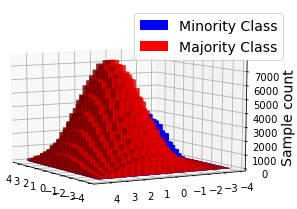
\includegraphics[width=\textwidth]{Undersampling_2D_OriginalDataset}
			         \caption{Original.}
			         \label{fig:Undersampling_2D_OriginalDataset}
			     \end{subfigure}
			     \hfill
			     \begin{subfigure}[b]{0.24\textwidth}
			         \centering
			         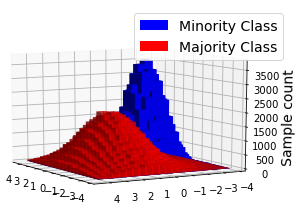
\includegraphics[width=\textwidth]{Undersampling_2D_UndersampledDataset}
			         \caption{Undersampled. $\beta=0.25$.}
			         \label{fig:Undersampling_2D_UndersampledDataset}
			     \end{subfigure}
			        \caption{Gaussian dataset.}
			        \label{fig:Undersampling_2D_OriginalHistograms}
			\end{figure}

	\subsubsection{Generalization Ability}
		Induction algorithms require a sufficient amount of data to learn a model that generalizes well.  If the training set is not large, a classifier may just memorize the characteristics of the training data. Moreover, undersampling has the potential of eliminating valuable samples from consideration of the classifier entirely \cite{undersampling_generalization}, so it may exacerbate this problem of lack of data. The obtained training set may vary greatly from one undersampling to another, which leads to a high variance on the learned model. Hence, the achievable complexity of the hypothesis set must be reduced to ensure a good generalization.
		
	\subsubsection{Posterior Bias}
		One goal of undersampling is to change the prior probabilities of the classes to make them more balanced. The classifier assumes that the features encountered at testing follow the same distribution as the training set. This mismatch introduced by design is known as sampling selection bias \cite{sampling_bias} on the posterior distribution.

		Let $(\mathcal{X}, \mathcal{Y})$ denote the pairs of feature vectors, $\mathbf{x} \in \mathbb{R}^n$,  and binary labels, $y \in \{0, 1\}$, contained in our original dataset. We assume that the number of samples labeled as zero is small compared with the number of samples in class one. Undersampling randomly removes points from the majority class. We describe this sampling with the binary random variable $S$, which takes the value 1 if a sample is selected.

		It is reasonable to assume that the selection is independent of the features given the class. Then, applying Bayes rule, the law of total probability and noting that the samples from the minority class are always selected, we obtain
		\begin{align*} \label{posterior}
			p' = & P(y=0|\mathbf{x}, s=1)=  \frac{P(s=1|y=0, \mathbf{x})P(y=0|\mathbf{x})}{P(s=1|\mathbf{x})}=\notag\\
					=&  \frac{P(y=0|\mathbf{x})}{P(y=0|\mathbf{x})+P(s=1|y=1)P(y=1|\mathbf{x})}=\notag\\
=&\frac{p}{p+\beta(1-p)},
		\end{align*}
where $p$ and $p'$ denote the posterior probability of encountering a sample from the minority class when employing the original and the undersampled dataset respectively. Whereas $\beta$ denotes the probability of keeping a sample from the majority class.


		The posterior is highly affected by the sampling rate. As more samples are removed, the classification is more biased towards the minority class. Figure \ref{fig:Undersampling_2D_Contour_Classification} shows the decision region of a naive Bayes classifier, where the area within each circle corresponds to the cluster of points classified as the minority class for a given undersampling rate. As the training set is undersampled the region of points that are labeled as the minority class grows. The undersampling rate not only influences the posterior bias, but also the algorithm's ability to generalize. Thus, $\beta$ should be chosen with care. Figure \ref{fig:F1_Score} presents the average F1-score over different training sets. We observe that the score is concave and in this case the optimum occurs with $\beta=0.67$, with a 2\% performance improvement.

			\begin{figure}[h]
				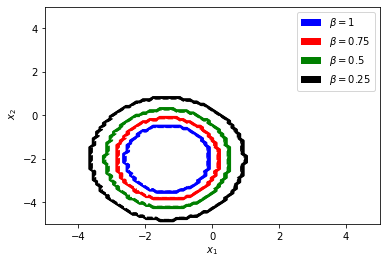
\includegraphics[scale=0.45]{Undersampling_2D_Contour_Classification}
				\centering
				\caption{Influence of undersampling on the classification region.}
				\label{fig:Undersampling_2D_Contour_Classification}
			\end{figure}
		
		\begin{figure}[h]
			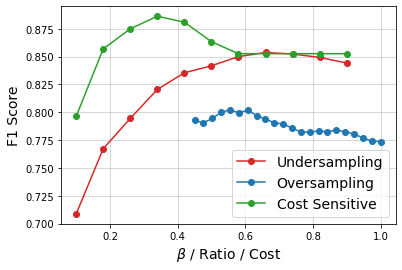
\includegraphics[scale=0.45]{F1_scores_dataset1}
			\centering
			\caption{F1-score vs. undersampling rate, oversampling rate and cost.}
			\label{fig:F1_Score}
		\end{figure}
		
		Another factor that strongly influences the posterior bias is class separability. The bias is higher when conditional distributions are similar across the classes\cite{undersampling_posterior}. To analyze this behavior we reduced the problem to a one-dimensional setting, the results are depicted in Figure \ref{fig:Undersampling_posterior}. We confirm that undersampling shifts the posterior distribution in favor of the minority class. Nevertheless, the shift caused by $\beta$ is lower under the configuration with lower overlap.

			\begin{figure}[h]
			     \centering
			     \begin{subfigure}[h]{0.24\textwidth}
			         \centering
			         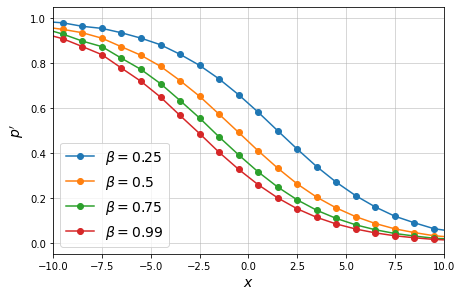
\includegraphics[width=\textwidth]{Undersampling_PosteriorBias}
			         \caption{$|\mu_0 - \mu_1|=3$.}
			         \label{fig:Undersampling_PosteriorBias}
			     \end{subfigure}
			     \hfill
			     \begin{subfigure}[h]{0.24\textwidth}
			         \centering
			         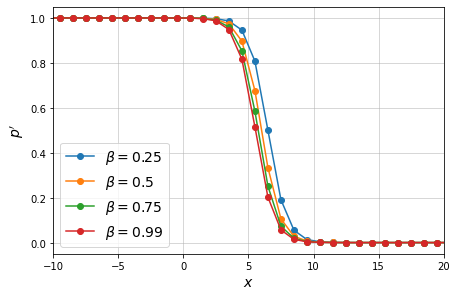
\includegraphics[width=\textwidth]{Undersampling_PosteriorBias_Separated}
			         \caption{$|\mu_0 - \mu_1|=13$.}
			         \label{fig:Undersampling_2D_UndersampledDataset}
			     \end{subfigure}
			        \caption{Influence of undersampling on posterior probability of the minority class.}
			        \label{fig:Undersampling_posterior}
			\end{figure}
		

	\subsection{Oversampling}
	
	Another technique to balance datasets is oversampling, that is, artificially creating new instances of the minority class. This can be done just by cloning existing samples, but this is not really adding new information to the model. More elaborated methods create samples by interpolation. The most widely used is the Synthetic Minority Oversampling Technique (SMOTE). It works by selecting a random sample, taking another nearby sample and creating points in between. This procedure is repeated multiple times until the desired amount of new samples is created.
	
	In Figure \ref{fig:Oversampling_2D_OriginalHistograms}, it is possible to observe the effect of oversampling on the 2D dataset. For the chosen ratio of 1, the number of samples of both classes is the same.
	
	
		\begin{figure}[h]
		\centering
		\begin{subfigure}[h]{0.24\textwidth}
			\centering
			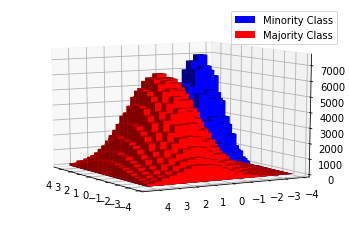
\includegraphics[width=\textwidth]{Oversampling_2D_OriginalDataset}
			\caption{Original.}
			\label{fig:Oversampling_2D_OriginalDataset}
		\end{subfigure}
		\hfill
		\begin{subfigure}[h]{0.24\textwidth}
			\centering
			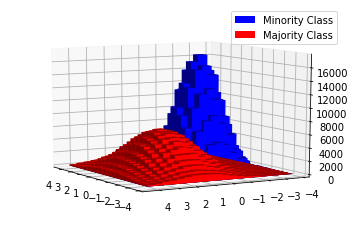
\includegraphics[width=\textwidth]{Oversampling_2D_OversampledDataset}
			\caption{Oversampled. Ratio=1.}
			\label{fig:Oversampling_2D_OversampledDataset}
		\end{subfigure}
		\caption{Gaussian dataset.}
		\label{fig:Oversampling_2D_OriginalHistograms}
	\end{figure}
	
	A sensitivity analysis for several ratios has been conducted and the optimum ratio is determined to be around 0.55, which means that the minority class is oversampled until the number of minority samples is 55\% of the samples of the majority class. The increase in F1 score for this ratio is almost 0.6\%, as shown in Figure \ref{fig:F1_Score}.


	\subsection{Cost-Sensitive Techniques}
	Unlike the data-level based methods seen above, cost-sensitive learning requires the training algorithm to be modified to include uneven penalizations when samples are misclassified. In other words, we are minimizing the risk based on an uneven loss function. Depending on the loss function that we choose, the risk function -- and therefore the estimated distribution parameter -- will impact the decision boundaries of the new cost-sensitive classifier. The loss function selected for this study is Weighted Likelihood (WL). This approach consists of weighting the training samples according to their cost of misclassification. The loss function and empirical risk become
	
	\begin{equation*}
	\begin{aligned} \label{costWL}
			L(y,\boldsymbol x, \theta) &= c(y)\mathbbm{1}\{ \hat y \neq y \} \\
			R^{WL}_{emp}(\theta) &= \int \int L(y,\boldsymbol x, \theta) p(\boldsymbol x, y) d\boldsymbol x \text{ }dy=\\
				      &=-\frac{1}{N} \sum_n c(y_n,\boldsymbol x_n,) \ln p(y_n | \boldsymbol x_n;\theta)
		\end{aligned},
	\end{equation*}
	
	where $L$ is the loss function, $R$ is the empirical risk, $c(y)$ is the cost of misclassifying class $y$, $\pi_k$ are the prior probabilities of each class and $\theta$ is the set of estimated classifier parameters. With this configuration, the decision rule of the Naive-Bayes classifier is
	
	$$ h^{NB}(\boldsymbol x) = \underset{k}{\operatorname{argmax}} \text{ } c(y_k) \pi_k p_{\boldsymbol x | y}(\boldsymbol x|y=k)$$
	
	Fig. \ref{fig:F1_Score} shows the results when different costs are applied to the Naive-Bayes classification. Note that this technique is especially effective when the penalization of the majority class is higher, leading to a F1-score improvement with respect to the symmetric loss function of 2\%.
	
\section{Classification Impact on Real Data}
The remainder of the paper studies the Twitter dataset. The first attempt was to use the same techniques as in the bi-dimensional dataset. Nevertheless, the presence of categorical variables makes oversampling and custom cost-sensitive approaches less suitable. Therefore, the first approach relied solely on undersampling and Naive Bayes. The Naive Bayes classifier achieved a F1-score of 29.73\% and including undersampling only improved the performance up to 41.98\%. The only solution is to use more complex classifiers that can cope with a dataset like this.

Ensemble Classifiers are known to improve the performance of single classifiers in imbalanced datasets \cite{ensembles_review} by combining separate weak learners into a composite whole. Both bagging and boosting algorithms have been implemented from scratch to explore their advantages and compare them with highly-effective classifiers such as XGBoost.

\subsection{Bagging}
Bagging algorithms are composed of two parts: bootstrapping and aggregation. The first part consists of selecting a subsample of the dataset. In bagging algorithms, weak learners are only trained over a fraction of the dataset. For training, decision tree classifiers are employed. Once all the classifiers are trained, the predictions of all the models are aggregated to provide the final prediction. Note that these algorithms are purely variance reducing procedures intended to mitigate instability, especially the one associated with decision trees.

\subsection{AdaBoost}
Unlike bagging, boosting fits the weak learners in an adaptive way: A different significance is assigned to each of the base learners based on the samples that were misclassified in the previous iteration. It was first introduced by Schapire in 1990, who proved in \cite{schapire} that a weak learner can be turned into a strong learner in the sense of probably approximately correct (PAC) learning framework. In particular, the AdaBoost algorithm stands out in the field of ensemble learning as one of the top ten data mining algorithms \cite{top10algo}. One of its main advantages is the versatility to incorporate cost-sensitive techniques. We implemented a custom AdaBoost classifier that enables us to gain control over the algorithm at a lower level, make adjustments when necessary and create other Adaboost-based classifiers such as AdaCost or Boosted SVM.

\begin{algorithm}
  \KwInput{Training set $D = \{x_i, y_i\}, i=1,\dots,N;$ and $y_i \in \{ -1,+1\}$; $T:$ Number of iterations; $I:$ Weak learner}
  \KwOutput{Boosted Classifier: $H(x)=sign\left( \sum^T_{t=1}\alpha_ih_t(x)\right)$ where $h_t, \alpha_t$ are the induced classifiers and their significance, respectively}
  %\KwData{Testing set $x$}
  $W_1(i) \leftarrow 1/N$ for $i=1,\dots,N$ %\tcp*{this is a comment}

  \tcc{Create a weak learner in each iteration}
  \For{t=1 to T}
    {
        $h_t \leftarrow I(D,W)$

        $\epsilon_t \leftarrow \sum^N_{i=1}W_t(i)[h_t(x_i)\neq y_i]$

        \If{$\epsilon_t > 0.5$}
        		{
		
		$T \leftarrow t-1$
		
		\bf{return}
		}
		
	$\alpha_t = \frac{1}{2}\ln \left( \frac{1-\epsilon_t}{\epsilon_t} \right)$
	
	\tcc{Update Weights}
	
	 $W_{t+1}(i) = W_t(i) e^{(-\alpha_th_t(x_i)y_i)}$ for $i=1,\dots,N$
	
	 Normalize $W_{t+1}$ such that $\sum^N_{i=1}W_{t+1}(i)=1$
	
    }
\caption{AdaBoost Algorithm}
\end{algorithm}

% Maybe we need to delete or reduce this paragraph
This custom implementation uses single decision trees with 2 leaf nodes. It takes the number of maximum iterations, namely the weak learners that will be fitted, and a dataset $D$ formed by N training samples, each constituted by a feature vector $\boldsymbol{x}_i$ and an associated binary label $y_i$. For each iteration, a weak classifier is created using the weighted training samples. In the first iteration, we allocate the same weight to all the samples, i.e. $1/N$. Once the decision tree has been created, we predict the class of the training samples and compute the weighted misclassification error $\epsilon_t$. Then, the significance $\alpha_t$ is calculated based on that error. Finally, the weights of each training sample are updated according to its significance and whether the sample was correctly classified or not. Note that the weights are increased by $e^{\alpha}$ if the sample is misclassified or decreased by $e^{-\alpha}$ if correctly classified, with  $\alpha_t \in [0,1]$ because $\epsilon_t \in [0,0.5]$.

AdaBoost uses all training samples to create each weak learner serially --in contrast to \textit{Bagging}, where \textit{bootstrap aggregating} is used to construct ensembles-- giving more focus to challenging instances and to turning the incorrect classifications into good predictions in the next iteration. Hence, AdaBoost can be considered as a "bias" reducing procedure, intended to increase the flexibility of stable (highly biased) weak learners when incorporated properly in a serial additive expansion. That is the reason why weak learners with a low variance but high bias --such as decision trees-- are well adapted for boosting. Lastly, the literature suggests that AdaBoost algorithms are generally resistant to overfitting regardless of the number of weak estimators employed. In fact, there are very few cases reported overfitting the training data \cite{BoostingStats}. This fascinating property is explained by 1) as the iterations proceed the weak learners tend to have less significance and 2) similarly to SVM, ensemble classifiers maximize the margin which allows promoting good generalization \cite{margin_adaboost}. The results section will further cover the impact of complexity on overfitting.

\subsection{AdaCost}
The AdaBoost algorithm is accuracy-oriented. In other words, it assumes each class has an even distribution. Therefore, in cases where the class distribution is uneven, the algorithm may incur systematic biases toward the majority class. Literature suggests two lines of work to incorporate an asymmetric weight update and eliminate these biases: \cite{need_boosting} 1) modify the model learned from data or 2) modifying how the model is used to make a decision. AdaCost falls into the former category, it aims at modifying the update of the weights based on a slight modification:
$$ W_{t+1}(i) = W_t(i) \exp \left(-\alpha_t y_i h_t(x_i) \boxed{\phi(i)} \text{ } \right),$$
with $$ W_1(i) = \frac{c_i}{\sum_{i=1}^Nc_i}$$
and where the new boxed term is called the cost-adjustment function. We use this function to allocate different penalizations across different classes. %This function is left for design since the literature suggest more than one alternatives.

In this project, we used the cost-adjustment function suggested in \cite{ensembles_review}:
$$\phi(i) = 0.5C_i \left( \mathbbm{1}\{ h_t(\boldsymbol x)=1\} -  \mathbbm{1}\{ h_t(\boldsymbol x)=-1\} \right)+0.5$$ where $C_i$ is a hyper-parameter that establishes the misclassification cost of the sample $i$, which ultimately depends upon the class of that sample. This cost-adjustment function yields to an upper bound cumulative misclassification cost equal to $d\prod_{t=1}^TZ_t$, where $d= \sum c_i$ and $Z_t$ is the sum of the costs calculated for $W_{t+1}$, i.e. the coefficient that we use to normalize the weights in AdaBoost \cite{adacost}. Since boosting minimizes $Z_t$, the significance ultimately needs to be updated in a different way \cite{improved_boosting}:
$$ \alpha = \frac{1}{2}\ln\frac{1+r}{1-r},\quad \text{where } r=\sum_iD(i)u_i, \  u_i=y_i h(x_i)\phi(i)$$.

All in all, the AdaCost algorithm follows the same procedure as AdaBoost with changes in the significance and weight update rule to incorporate an asymmetric penalization cost.

\subsection{AdaMEC}
The AdaMEC algorithm falls into the second category introduced in the previous part. The model is trained with the original AdaBoost, but modifies the decision rule by exploiting the Bayesian decision theory:
$$ H_{AdaMEC}(\boldsymbol x) = sign \left( \sum_{y \in \{-1,+1\}} c(y) \sum_{\tau: h_{\tau}(\boldsymbol x)=y} \alpha_{\tau} h_{\tau}(\boldsymbol x)\right)$$

This is called the Minimum Expected Cost rule and it assumes that the weighted votes of each weak learner are proportional to the class probabilities. We have incorporated this classifier in this study because it has been reported as one of the best cost-sensitive AdaBoost classifiers \cite{need_boosting}.


\subsection{Boosting SVM}
One of the practical concerns about AdaBoost is the accuracy/diversity dilemma \cite{study_boosted_svm}: when the weak learners are actually strong classifiers and they do not disagree too much on their vote, the performance of boosting is weakened. Support vector machines (SVM) are known to be strong learners that minimize structural risk such that they should not work well when embedded. However, the work on \cite{study_boosted_svm} and \cite{boosting_svm} suggests that if properly weakened, Boosted SVM can exceed the classification performance of traditional SVMs or AdaBoost on imbalanced datasets, and gain control over the accuracy/diversity issue. To do that, we have used radial basis function kernel (RBF), which uses the Gaussian width $\sigma$ to map the features on a high dimensional feature space. The performance of RBFSVM can be conveniently controlled by adjusting $\sigma$. Large values of sigma will lead to very weak classifiers. Algorithm 2 gives a detailed description of the implementation.

\begin{algorithm}

 \KwInput{Training set $D = \{x_i, y_i\}, i=1,\dots,N;$ and $y_i \in \{ -1,+1\}$; $T:$ Maximum number of iterations; The initial $\sigma=\sigma_{ini}, \sigma_{min}, \sigma_{step}$}
\KwOutput{Boosted Classifier: $H(x)=sign\left( \sum^T_{t=1}\alpha_ih_t(x)\right)$ where $h_t, \alpha_t$ are the induced classifiers and their significance, respectively}
  %\KwData{Testing set $x$}
  $W_1(i) \leftarrow 1/N$ for $i=1,\dots,N$ %\tcp*{this is a comment}

  \tcc{Create a weak learner in each iteration}
  \While{$\sigma > \sigma_{min}$ and $t<T$}
    {
        $t \leftarrow t+1$

        $h_t \leftarrow RBFSVM(D,W,\sigma)$ \tcp*{Train RBFSVM}

        $\epsilon_t \leftarrow \sum^N_{i=1}W_t(i)[h_t(x_i)\neq y_i]$

        \If{$\epsilon_t > 0.5$}
        		{
		
		$\sigma \leftarrow \sigma - \sigma_{step}$
		
		}
	\Else
	{
	$\alpha_t = \frac{1}{2}\ln \left( \frac{1-\epsilon_t}{\epsilon_t} \right)$
	
	\tcc{Update Weights}
	
	 $W_{t+1}(i) = W_t(i) e^{(-\alpha_th_t(x_i)y_i)}$ for $i=1,\dots,N$
	
	 Normalize $W_{t+1}$ such that $\sum^N_{i=1}W_{t+1}(i)=1$
	 }
    }
\caption{Boosted SVM Algorithm}
\end{algorithm}

The main disadvantage of SVM is that the running time to train the model does not scale well with the size of the training set\cite{boosting_svm}. Our training set has more than 30,000 samples so the training would take a significant amount of time. Therefore, a preprocessing step was applied to the training data, whose dimensionality is reduced using PCA and ultimately under-sampled to speed-up the training process.

\subsection{XGBoost}
Nowadays, XGBoost is one of the most effective classification algorithms. In fact, it has been the winner of many competitions in the last years \cite{xgboost}. The working principle is additive tree learning, which means that the knowledge acquired on an iteration is used to train the following tree of the model. This new tree has to minimize the objective function that includes a training loss and a regularization term. The second-order Taylor expansion is employed, as the actual function can be very complex. The structure of the new tree is optimized to produce the maximum reduction of the objective function. The tree split that gives the maximum similarity between its prediction and the output is added. 

In practice, XGBoost is the classification algorithm that achieves the highest F1-score and accuracy. The XGBoost library is used to train this algorithm for our dataset.

\section{Results and Discussion}
This section discusses the performance of each classifier, addresses how these algorithms work for different imbalance rates and shows how the number of learners affects the true and empirical risks.

\subsection{Performance Results}

The performance results of each methodology are summarized in Table \ref{tab:PerformanceComparison}. It includes the F1-score, accuracy, precision, recall and AUC in order to compare the algorithms from multiple perspectives. All scores have been obtained with classifiers that had 100 weak learners.

\begin{table}[htbp]
\caption{Best Classification Performances}

\begin{center}

\begin{tabular}{|c|c|c|c|c|c|c|}

\hline
\textbf{Type of} & & \multicolumn{5}{|c|}{\textbf{Scores (\%)}} \\
\cline{3-7}

\textbf{Method} & \textbf{Classifier} &\textbf{\textit{F-1}}& \textbf{\textit{Acc.}}&\textbf{\textit{Prec.}}&\textbf{\textit{Rec.}}&\textbf{\textit{AUC}}\\
\hline

& AdaBoost$^*$ &68.68&84.55&74.43&63.75&77.91  \\
\cline{2-7}

& Bagging$^*$ &49.98&78.03&63.27&41.31&66.31  \\
\cline{2-7}

Ensemble & R. Forest &27.73&76.96&83.33&26.63&57.71  \\
\cline{2-7}

& BoostSVM$^*$$^*$ &62.18&73.42&53.91&73.42&0.5  \\
\cline{2-7}

& XGBoost  &\textbf{76.70}&\textbf{88.63}&\textbf{84.18}&\textbf{70.44}&\textbf{82.82} \\
\hline

Cost & AdaCost$^*$ &59.53&80.70&67.23&53.42&72.00  \\
\cline{2-7}

Sensitive& AdaMEC &70.99&85.88&78.21&64.99&79.21  \\
\hline

& AdaBoost$^*$ &69.03&83.14&67.42&70.71&79.17  \\
\cline{2-7}

& Bagging$^*$ &59.27&75.90&53.80&65.99&72.74  \\
\cline{2-7}

Hybrid & R. Forest &60.82&80.83&66.54&56.01&72.91  \\
\cline{2-7}

sampling)& XGBoost  &76.69&87.89&78.49&74.97&83.76 \\
\cline{2-7}

 & AdaCost$^*$ &57.51&79.29&63.24&52.72&70.82  \\
\cline{2-7}

& AdaMEC &70.97&84.62&71.19&70.75&80.19  \\
\hline

\multicolumn{4}{l}{$^{\mathrm{*}}$Custom implementation.}
\multicolumn{4}{l}{$^{\mathrm{*}}$$^{\mathrm{*}}$Metrics are weighted.}

\end{tabular}

\label{tab:PerformanceComparison}
\end{center}
\end{table}

Under the category of ensemble  algorithms, XGBoost outperforms every other algorithm in all metrics. Looking at the F1-score, XGBoost is close to 80\%. The next algorithm is AdaBoost, whose F1-score is above 68\%. The rest of the ensemble classifiers are clearly inferior. Regarding cost-sensitive algorithms, for this particular dataset, they do not give any substantial advantage. Only AdaMEC is slightly better than the original AdaBoost. For hybrid algorithms, which combine ensemble and cost-sensitive algorithms plus undersampling, the optimum beta (the one that gives the maximum F1-score) for each algorithm is selected. A few of the classifiers improve, as is the case of Random Forest, Bagging and AdaBoost. However, XGBoost still has the largest F1-score.

\subsection{Impact of Imbalance Data on Classification}

This section studies how each algorithm works if fewer samples of the majority class are considered (conceptually, this is similar to undersampling the majority class). Figure \ref{Fig:ImbalanceComparison} shows the performance of each algorithm for different rates. For example, the rate of 0.5 implies that the number of majority and minority class samples are the same.

\begin{figure}[htbp]
\centerline{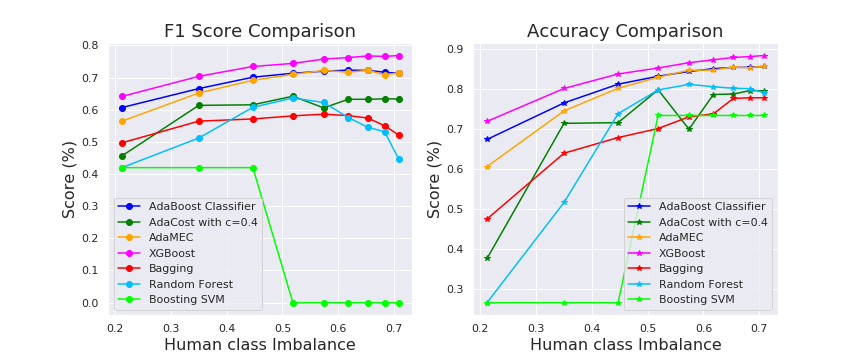
\includegraphics[scale=0.35]{pictures/Imbalance_Comparison.png}}
\caption{Impact of imbalanced training set on classification.}
\label{Fig:ImbalanceComparison}
\end{figure}

It is really interesting to see that some of the algorithms have a peak in the F1-score metric when rates around 0.6 are considered. Random Forest has a strong peak on 0.52 that supports why in the previous section this algorithm improves a 30\% in its F1-score when the undersampling is included. Bagging has the same effect, increasing around a 10\% when the optimum undersampling is applied.  


\subsection{Overfitting Analysis}

Figure \ref{fig:True_empirical_risk_complexity} shows the evolution of both empirical and true risk for increasing algorithm complexity. The true risk and the empirical risk were computed with a validation and training set, respectively. Complexity increases with the number of learners trained by the algorithm, as it involves a larger number of hypotheses. We conclude that XGBoost is the algorithm that minimizes the true risk. Even with just a few estimators, it is better than any other algorithm. The true risk rapidly decreases as the number of learners grows, up until 50 learners when a risk below 12\% is achieved.

\begin{figure}
	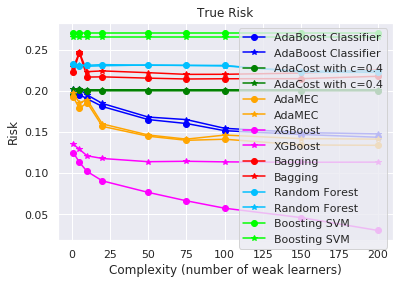
\includegraphics[scale=0.45]{True_empirical_risk_complexity}
	\centering
	\caption{True (triangles) and empirical (circles) risks vs. complexity.}
	\label{fig:True_empirical_risk_complexity}
\end{figure}

Regarding other algorithms, AdaBoost and AdaMEC tend to become similar as the number of weak learners increases. Although not comparable to XGBoost, both performances are satisfactory. However, AdaMEC seems to outperform AdaBoost. Regarding AdaCost, Bagging and Random Forest, their true risks are comparably high, and their performance does not improve much with the number of learners.

It is worth noting that the true risk remains stable after a certain number of learners, while the empirical risk always seems to decrease. This is especially visible in XGBoost. This occurs because the algorithm learns patterns that are extremely specific to the training set, but which are not generalizable to the test set. Therefore, very few improvements are seen on the true risk. %In the other algorithms, the different between empiricial and true risk is not as significant, but the true risk always remain higher than the empirical risk.

%\subsection{Diversity Analysis}

%Chart of Accuracy vs. Diversity
% Mirar Fig. 3 de esta paper: http://users.cecs.anu.edu.au/~wanglei/My_papers/AdaBoost_SVM_IJCNN_2005.pdf

\section{Conclusions}
This paper shows how the classification of imbalanced datasets can be addressed. Some methods that change the dataset on a data level, such as oversampling or undersampling, while others develop more complex classifiers (cost-sensitive and ensemble methods). In the synthetic Gaussian dataset, the first type of methods was employed with satisfactory results and the F1-score is higher. However, applying the same methods to the Twitter dataset did not yield a significant improvement. Consequently, several ensemble and hybrid classifiers have been tested, including some custom implementations. It has been determined that a substantial improvement of almost 30\% on the F1-score can be achieved in relation to a Naive Bayes classifier with undersampling. The ensemble and cost-sensitive classifiers that give the maximum F1-score are the XGBoost and AdaMEC, respectively. Among the ensemble algorithms, it has been shown that boosting algorithms are superior to bagging algorithms%, which are the other type of ensemble algorithms
. For this particular dataset, some hybrid methods (including undersampling of the majority class) are more effective than the corresponding default ensemble and cost-sensitive methods. This is the case of Bagging and Random Forest. In addition, this paper has also explored the versatility of these algorithms against the number of weak-learners and the rate of imbalance in the dataset. It was determined that XGBoost is the most resilient to imbalance rates and it has the lowest empirical and true in a broad spectrum of weak learners.

\vspace{12pt}

\begin{thebibliography}{1}

\bibitem{data_imbalance_overview}
 V.~S. {Spelmen} and R.~{Porkodi}, ``A review on handling imbalanced data,'' in
   {\em 2018 International Conference on Current Trends towards Converging
   Technologies (ICCTCT)}, pp.~1--11, 2018.

 \bibitem{undersampling_generalization}
 M.~{Wasikowski} and X.~{Chen}, ``Combating the small sample class imbalance
   problem using feature selection,'' {\em IEEE Transactions on Knowledge and
   Data Engineering}, vol.~22, no.~10, pp.~1388--1400, 2010.

 \bibitem{sampling_bias}
 Q.-C. Joaquin, {\em Dataset shift in machine learning}.
 \newblock MIT, 2009.

 \bibitem{undersampling_posterior}
 A.~D. {Pozzolo}, O.~{Caelen}, R.~A. {Johnson}, and G.~{Bontempi}, ``Calibrating
   probability with undersampling for unbalanced classification,'' in {\em 2015
   IEEE Symposium Series on Computational Intelligence}, pp.~159--166, 2015.

 \bibitem{ensembles_review}
 M.~{Galar}, A.~{Fernandez}, E.~{Barrenechea}, H.~{Bustince}, and F.~{Herrera},
   ``A review on ensembles for the class imbalance problem: Bagging-, boosting-,
   and hybrid-based approaches,'' {\em IEEE Transactions on Systems, Man, and
   Cybernetics, Part C (Applications and Reviews)}, vol.~42, no.~4,
   pp.~463--484, 2012.
   
 \bibitem{improved_boosting}
 Schapire, Robert E. and Yoram Singer, "Improved boosting algorithms using confidence-rated predictions,", Springer Netherlands, 1999.
 
\bibitem{adacost}
  Fan, Wei and Stolfo, Salvatore and Zhang, Junxin and Chan, Philip,
  "AdaCost: Misclassification Cost-sensitive Boosting,"
  {\em Proceedings of the Sixteenth International Conference on Machine Learning (ICML'99)}
  
\bibitem{boosting_svm}
   Elkin Garc{\'{\i}}a and Fernando Lozano,
   "Machine Learning and Data Mining in Pattern Recognition,"
   {\em 5th International Conference, {MLDM} 2007}, Leipzig, Germany, July 18-20, 2007, Post Proceedings
   
\bibitem{study_boosted_svm}
    {Xuchun Li} and {Lei Wang} and E. {Sung},
    "A study of AdaBoost with SVM based weak learners,"
    {\em Proceedings. 2005 IEEE International Joint Conference on Neural Networks}, 2005.
    
\bibitem{need_boosting}
Nikolaou, Nikos and Edakunni, Narayanan and Kull, Meelis and Flach, Peter and Brown, Gavin, 
"Cost-sensitive boosting algorithms: Do we really need them?," Vol. 104, 2016.


\bibitem{margin_adaboost}
Rudin, Cynthia and Daubechies, Ingrid and Schapire, Robert,
 "The Dynamics of AdaBoost: Cyclic Behavior and Convergence of Margins,"
 {\em Journal of Machine Learning Research}, 2004.
 
\bibitem{top10algo}
Wu, Xindong and Kumar, Vipin and Quinlan, Ross and Ghosh, Joydeep and Yang, Qiang and Motoda, Hiroshi and Mclachlan, G. and Ng, Shu Kay Angus and Liu, Bing and Yu, Philip and Zhou, Zhi-Hua and Steinbach, Michael and Hand, David and Steinberg, Dan,
"Top 10 algorithms in data mining," {\em {Knowledge and Information Systems}}, Vol. 14, 2007.

\bibitem{BoostingStats}
Jerome Friedman and Trevor Hastie and Robert Tibshirani,
"Additive Logistic Regression: a Statistical View of Boosting,"
{\em Annals of Statistics}, Vol. 28, 1998.

\bibitem{schapire}
Schapire, Robert E.,
"The Strength of Weak Learnability," Vol. 5, 1990. 

\bibitem{xgboost}
T. {Chen} and C.~{Guestrin}, ``XGBoost: A Scalable Tree Boosting System,'' in
{\em Proceedings of the 22nd ACM SIGKDD International Conference on Knowledge Discovery and Data Mining}, pp.~785--794, 2016.
   
\end{thebibliography}

%\bibliographystyle{ieeetr} 
%\bibliography{ref2.bib}
%\bibliography{ECE6254_references.bib}
\end{document}
